\documentclass[a4paper, 11pt]{scrartcl}

\usepackage[ngerman]{babel}
\usepackage[T1]{fontenc}
\usepackage[utf8]{inputenc}
\usepackage[a4paper, margin=2.5cm]{geometry}
\usepackage{amsmath}
\usepackage{amssymb}
\usepackage{graphicx}
\usepackage{hyperref}
\usepackage{wrapfig}

\newcommand{\vect}[2]{\begin{pmatrix}#1\\#2\end{pmatrix}}
\DeclareMathOperator{\atantwo}{atan2d}

\begin{document}

%%todo gute Überleitung / Anknüpfung an verwendetes mathematisches Modell

\section{Herleitung mathematischer Grundlagen}

\subsection{Herleitung der Formeln}\label{sec:herleitung}
%TODO gute Überleitung / Anknüpfung an verwendetes mathematisches Modell

%TODO bessere Überschrift: Grundlegend verwendete Prozedur zur Reflektion von eines Strahls
\subsubsection{Reflexion an einer Geraden}
Durch die Verwendung der Vektorrechnung lässt sich für unsere Arbeit die Reflexion eines Strahls an einer beliebigen regelmäßigen Geometrie auf die Reflexion eines Strahls an einer Geraden zurückführen. 
Diese ist damit ein essenzieller Prozess, der häufig durchgeführt werden muss.\\
\begin{wrapfigure}{rH}{10.5cm}
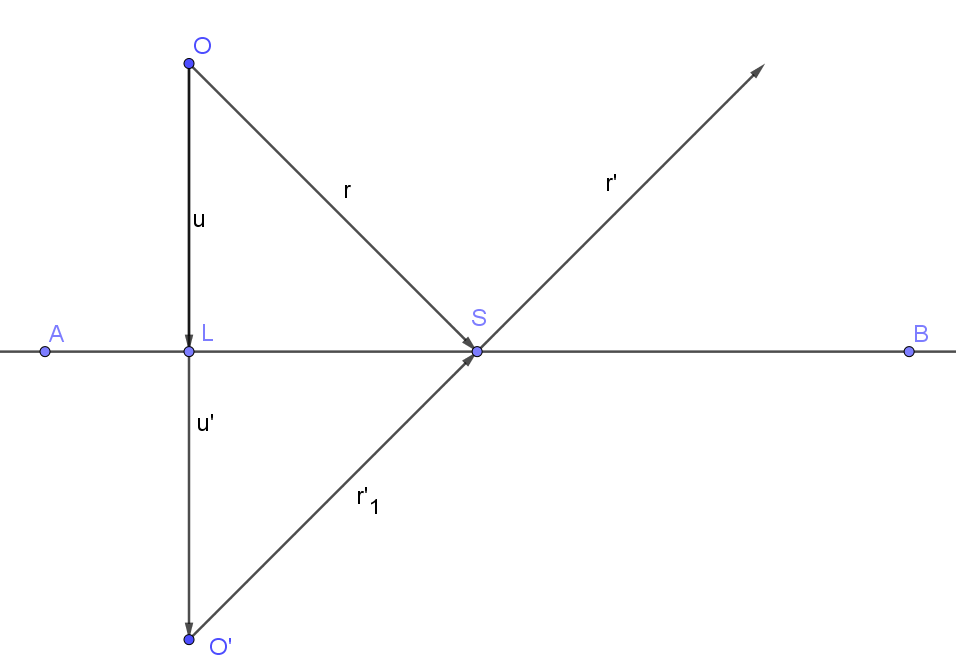
\includegraphics[scale=0.4]{pictures/LineRef.png}
\caption{Reflexion an einer Geraden}
%TODO caption
\end{wrapfigure}
Um die Berechnung des reflektierten Strahls durchzuführen müssen sowohl zwei Punkte der Geraden, $A$ und $B$, gegeben sein, sowie der Ausgangspunkt $O$ und der Richtungsvektor $\vec{r}$ des Ausgangsstrahls. 
Mittels des Vektors $\vec{u} = 2\cdot\overrightarrow{OL}$ zwischen $O$ und dem Lotfußpunkt $L$ von $O$ auf $\overline{AB}$ ergibt sich auch $\vec{o'} = \vec{o} + 2\cdot\vec{u}$ und damit der Spiegelpunkt $O'$ von $O$ an $AB$.
Weiterhin ist der Schnittpunkt $S$ des Strahls von $O$ in Richtung $\vec{r}$ mit der Geraden $AB$ durch die Formel\\
\begin{center}
$\vec{s} = \vec{o} - \dfrac{O_x \cdot \vec{r}_y - O_y \cdot \vec{r}_x - A_x \cdot \vec{r}_y - A_y \cdot \vec{r}_x}{A_x \cdot \vec{r}_y - A_y \cdot \vec{r}_x - B_x \cdot \vec{r}_y + B_y \cdot \vec{r}_x} \cdot \vec{r}$
\end{center}
bestimmt. 
Daraus ergibt sich folgend der Vektor\\
\begin{center}
$\vec{r'} = \vec{r'_1} = \overrightarrow{O'S}$
\end{center}
und damit auch der neue Strahl von $S$ in Richtung $r'$.


%TODO Überschrift
\subsubsection{Reflexion an weiteren regelmäßigen Geometrien}
Neben der Reflexion der Strahlen an einer einfachen Geraden haben wir uns auch entschieden, dies für Kreise, Kreisbögen und Ovale herzuleiten und zu implementieren. 
Grundsätzlich erfolgt dabei auch die Reflexion an einer Geraden, doch diese muss in Abhängigkeit der Form erst einmal bestimmt werden. 
Für folgende Herleitungen wird erneut von einem Strahl, der in $O$ beginnt und sich in Richtung $\vec{r}$ ausbreitet, ausgegangen.
\newpage
\begin{wrapfigure}{rH}{10.5cm}
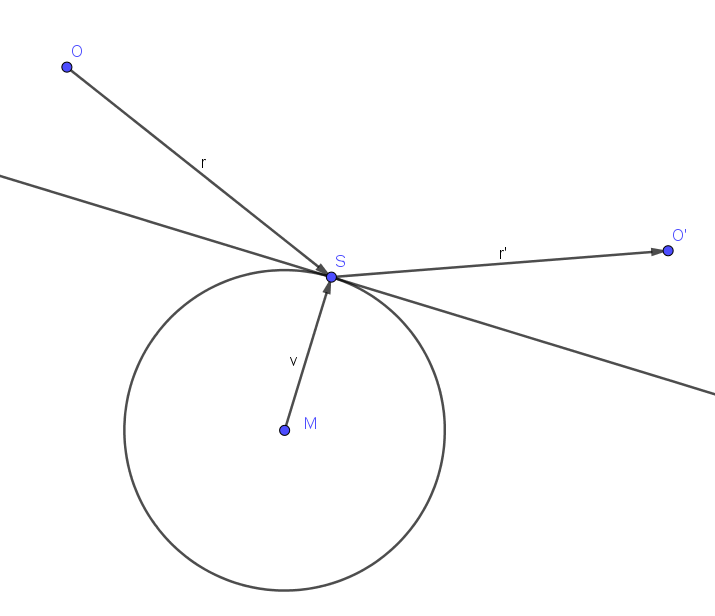
\includegraphics[scale=0.5]{pictures/CircleRef.png}
\caption{Reflexion an einem Kreis}
%TODO caption
\end{wrapfigure}
%old Um eine Berechnung daran zu ermöglichen, muss ein Kreis zunächst vektoriell dargestellt werden. 
Um die Berechnung an einem Kreis durchzuführen muss dieser zunächst vektoriell dargestellt werden.
Dies geschieht in der Form $K: \vec{x} = \vec{m} + \vec{v}$, wobei $\vec{m}$ der Ortsvektor zum Kreismittelpunkt $M$ und $\vec{v}$ der Richtungsvektor ist. 
Für letzteren gilt $\vec{v}_x^{~2} + \vec{v}_y^{~2} = r^2$, das heißt, dass jeder mögliche Richtungsvektor des Kreises $K$ ein Radius desselben ist. 
Mithilfe dessen wird zunächst der Punkt bestimmt, in welchem der Strahl den Kreis schneidet, indem das folgende Gleichungssystem nach den drei unbekannten Variablen $\lambda$, $\vec{v}_x$, $\vec{v}_y$ gelöst wird:
\begin{equation*}
\begin{split}
\vec{k}_x + \vec{v}_x & = O_x + \lambda\cdot\vec{r}_x\\
\vec{k}_y + \vec{v}_y & = O_y + \lambda\cdot\vec{r}_y\\
r^2 & = \vec{v}_x^{~2} + \vec{v}_y^{~2} 
\end{split}
\end{equation*}
Das so ermittelte $\lambda$ wird in die Formel $\vec{s} = \vec{o} + \lambda \cdot \vec{r}$  eingesetzt, um den Schnittpunkt $S$ zu berechnen. 
%oldDurch diesen wird anschließend eine Tangente gelegt, welche sich leicht über den Vektor $\vec{n} = \vec{MS}$ zwischen Kreismittelpunkt und Schnittpunkt ermitteln lässt. 
Durch den Vektor $\vec{n} = \vec{MS}$ zwischen Kreismittelpunkt und Schnittpunkt lässt sich leicht die Tangente in $S$ mit $T: ~\vec{x} = \vec{s} + \lambda \cdot \begin{pmatrix} -ny \\ nx \end{pmatrix}$ ermitteln.
Somit kann die Reflexion am Kreis auf eine Reflexion an einer Geraden zurückgeführt werden.\\
Die Reflexion an Kreisbögen funktioniert analog, aus einem Kreisbogen wird der entsprechende vollständige Kreis gebildet, an welchem wie beschrieben reflektiert wird. 
Jedoch muss zusätzlich noch überprüft werden, ob der Schnittpunkt mit dem \glqq Hilfskreis\grqq{} auch auf dem Teil des Kreises liegt, den dieser mit dem Kreisbogen teilt. 
Dies geschieht derart, dass festgestellt wird, ob der Winkel des Kreissektors von Startpunkt des Kreisbogens bis zum Schnittpunkt kleiner ist als der Winkel des Kreissektors, welchem der Kreisbogen insgesamt entspricht. 
Dazu wird eine Formel zur Berechnung des Winkels in mathematisch positiver Richtung von einem Vektor $v$ zu einem anderen Vektor $w$ $\sphericalangle(\vec{v}, \vec{w}) = -\atantwo(\vec{v}_x\cdot\vec{w}_y-\vec{v}_y\cdot\vec{w}_x,~\vec{v}_x\cdot\vec{w}_x+\vec{v}_y\cdot\vec{w}_y)$  verwendet.
\par
\begin{wrapfigure}{rH}{8cm}
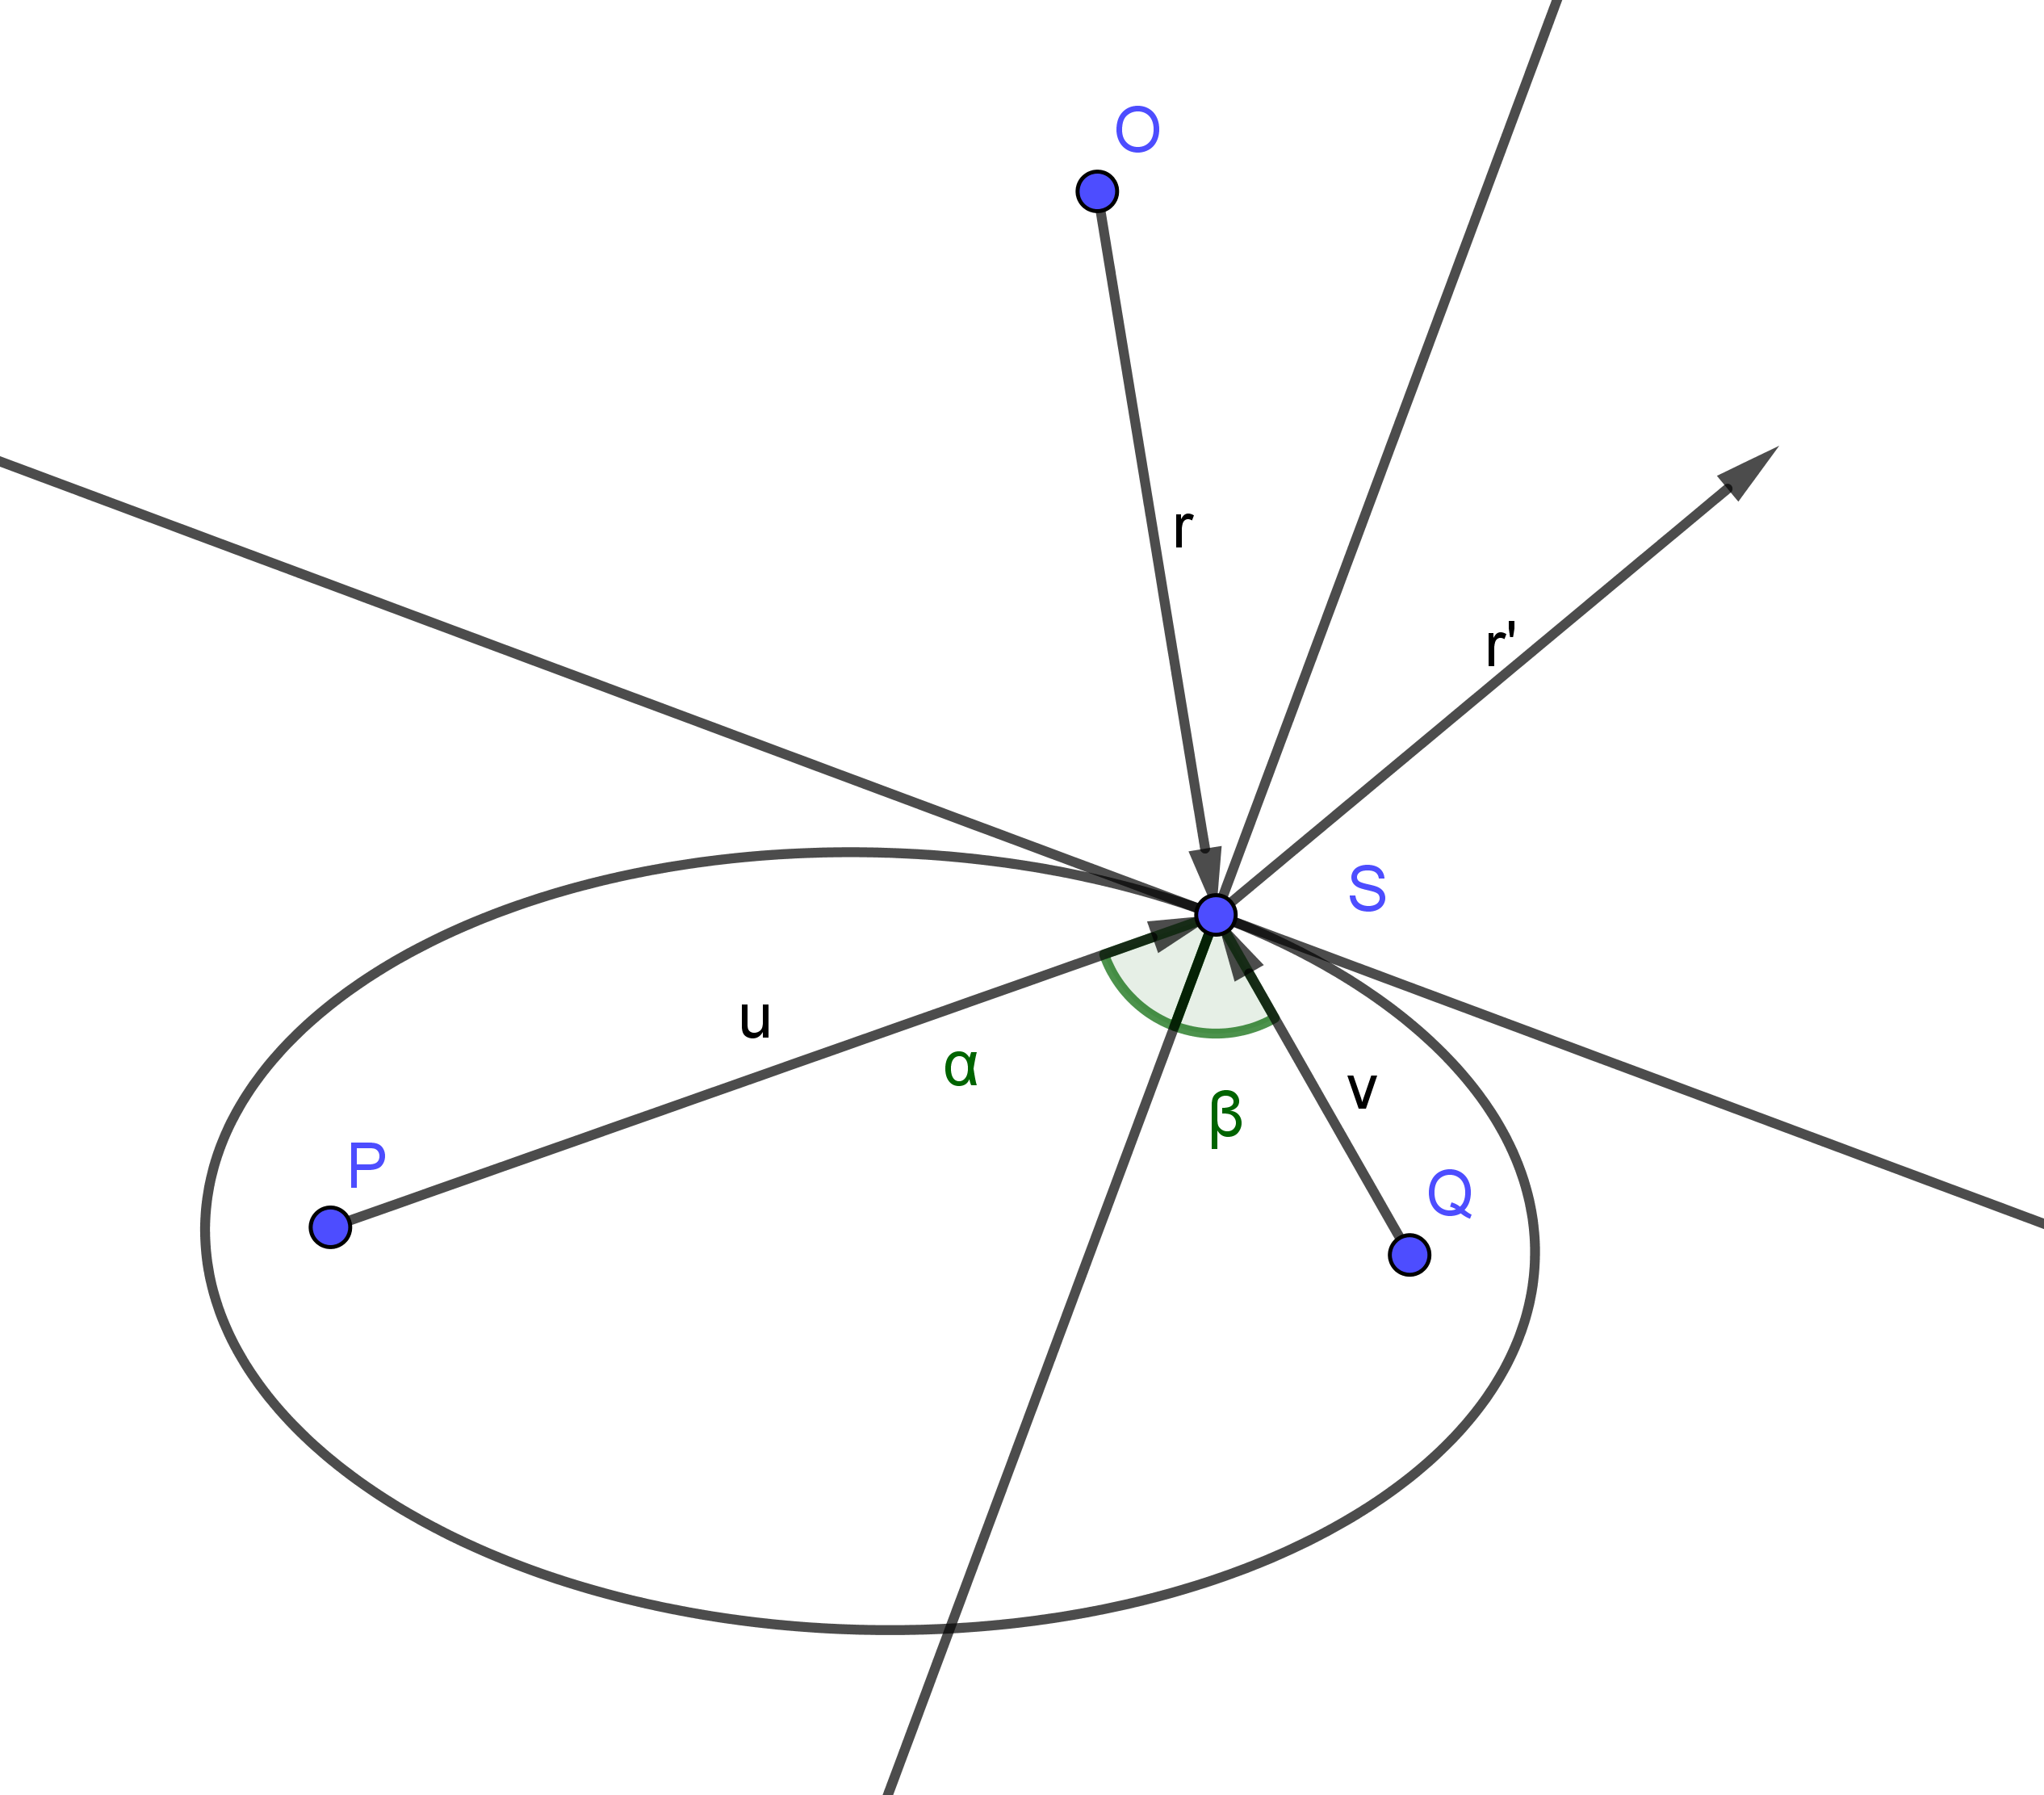
\includegraphics[scale=0.7]{pictures/OvalRef.png}
\caption{Reflexion an einer Ellipse}
%TODO caption
\end{wrapfigure}
%oldAls letzte von uns implementierte geometrische Form ist die Ellipse diejenige mit der aufwändigsten Berechnungsformel. 
Als letzte Form haben wir die Ellipse $E(P, Q, e)$ implementiert.
Wie beim Kreis ist es nötig, eine vektorielle Darstellung zu finden. 
Aufgrund der Definition einer Ellipse lautet diese $E: \vec{x} = \vec{p} + \vec{u} = \vec{q} + \vec{v}$ mit $ e = |\vec{u}| + |\vec{v}|$.
Zur Bestimmung des Schnittpunkts $S$ wird nun folgendes Gleichungssystem nach



%%todo Erwähnung weiterer Herleitungen im Anhang
% Erwähnung Quellen / Standardwissen
% Bezug auf gerichteten Winkel

%\subsection{Reflektion an Kreisbögen}

%\subsection{Reflektion an Ovalen}

%\subsection{Reflektion in Ecken}

\end{document}